%% LaTeX Beamer presentation template (requires beamer package)
%% see http://bitbucket.org/rivanvx/beamer/wiki/Home
%% idea contributed by H. Turgut Uyar
%% template based on a template by Till Tantau
%% this template is still evolving - it might differ in future releases!

\documentclass{beamer}
\usepackage[utf8]{inputenc}
\usepackage{etex}

\mode<presentation>
{
\usetheme{Boadilla}
%\usetheme{Warsaw}
\usecolortheme{wolverine}

\setbeamerfont{title}{shape=\itshape,family=\rmfamily}
\usefonttheme{serif}

\setbeamercovered{transparent}
}

\usepackage[english]{babel}

% font definitions, try \usepackage{ae} instead of the following
% three lines if you don't like this look
\usepackage{mathptmx}
\usepackage[scaled=.90]{helvet}
\usepackage{courier}
\usepackage{color}

\usepackage[T1]{fontenc}
%\usepackage{pictex}
%\usepackage{dsfont}
%\usepackage{ulem}

\title{CPCC Simulator}

%\subtitle{}

% - Use the \inst{?} command only if the authors have different
%   affiliation.
%\author{F.~Author\inst{1} \and S.~Another\inst{2}}
\author{Clemens Krainer}

% - Use the \inst command only if there are several affiliations.
% - Keep it simple, no one is interested in your street address.
\institute[University of Salzburg]
{
Department of Computer Sciences\\
University of Salzburg, Austria
}

\date{March 21, 2012}


% This is only inserted into the PDF information catalog. Can be left
% out.
\subject{Talks}



% If you have a file called "university-logo-filename.xxx", where xxx
% is a graphic format that can be processed by latex or pdflatex,
% resp., then you can add a logo as follows:

% \pgfdeclareimage[height=0.5cm]{university-logo}{university-logo-filename}
% \logo{\pgfuseimage{university-logo}}



% Delete this, if you do not want the table of contents to pop up at
% the beginning of each subsection:
%\AtBeginSubsection[]
%{
%\begin{frame}<beamer>
%	\frametitle{Outline}
%	\tableofcontents[currentsection,currentsubsection]
%\end{frame}
%}

% If you wish to uncover everything in a step-wise fashion, uncomment
% the following command:

%\beamerdefaultoverlayspecification{<+->}

\begin{document}

\begin{frame}
	\titlepage
\end{frame}

\begin{frame}
	\frametitle{Outline}
	\tableofcontents
% You might wish to add the option [pausesections]
\end{frame}


\section{Introduction}

%\subsection[Short First Subsection Name]{First Subsection Name}

\begin{frame}\frametitle{Introduction} %\framesubtitle{Task}
Task:
        \begin{itemize}
                \item simulation of physical helicopter swarms
                \item simulation of sensors
                \item abstraction of virtual vehicles (virtual helicopters)
                \item migration of virtual vehicles among flying physical helicopters
        \end{itemize}
\pause
\vspace{0.5cm}
Project Scope:
        \begin{itemize}
                \item real vehicles (physical helicopters) follow strict flight plans
                \item no network bandwith limits
                \item no processing power limits
        \end{itemize}
\end{frame}


\begin{frame}\frametitle{Introduction}
Applied Technologies:
        \begin{itemize}
                \item HTTP as protocol for sensor abstraction and data exchange
                \item Java as programming language
                \item software implemented as web applications
%               \item Apache Tomcat as web server and servlet container
        \end{itemize}
\end{frame}


\section {Simulator Overview}

\begin{frame}\frametitle{Simulator Overview}\framesubtitle{System}
        \begin{center}
                {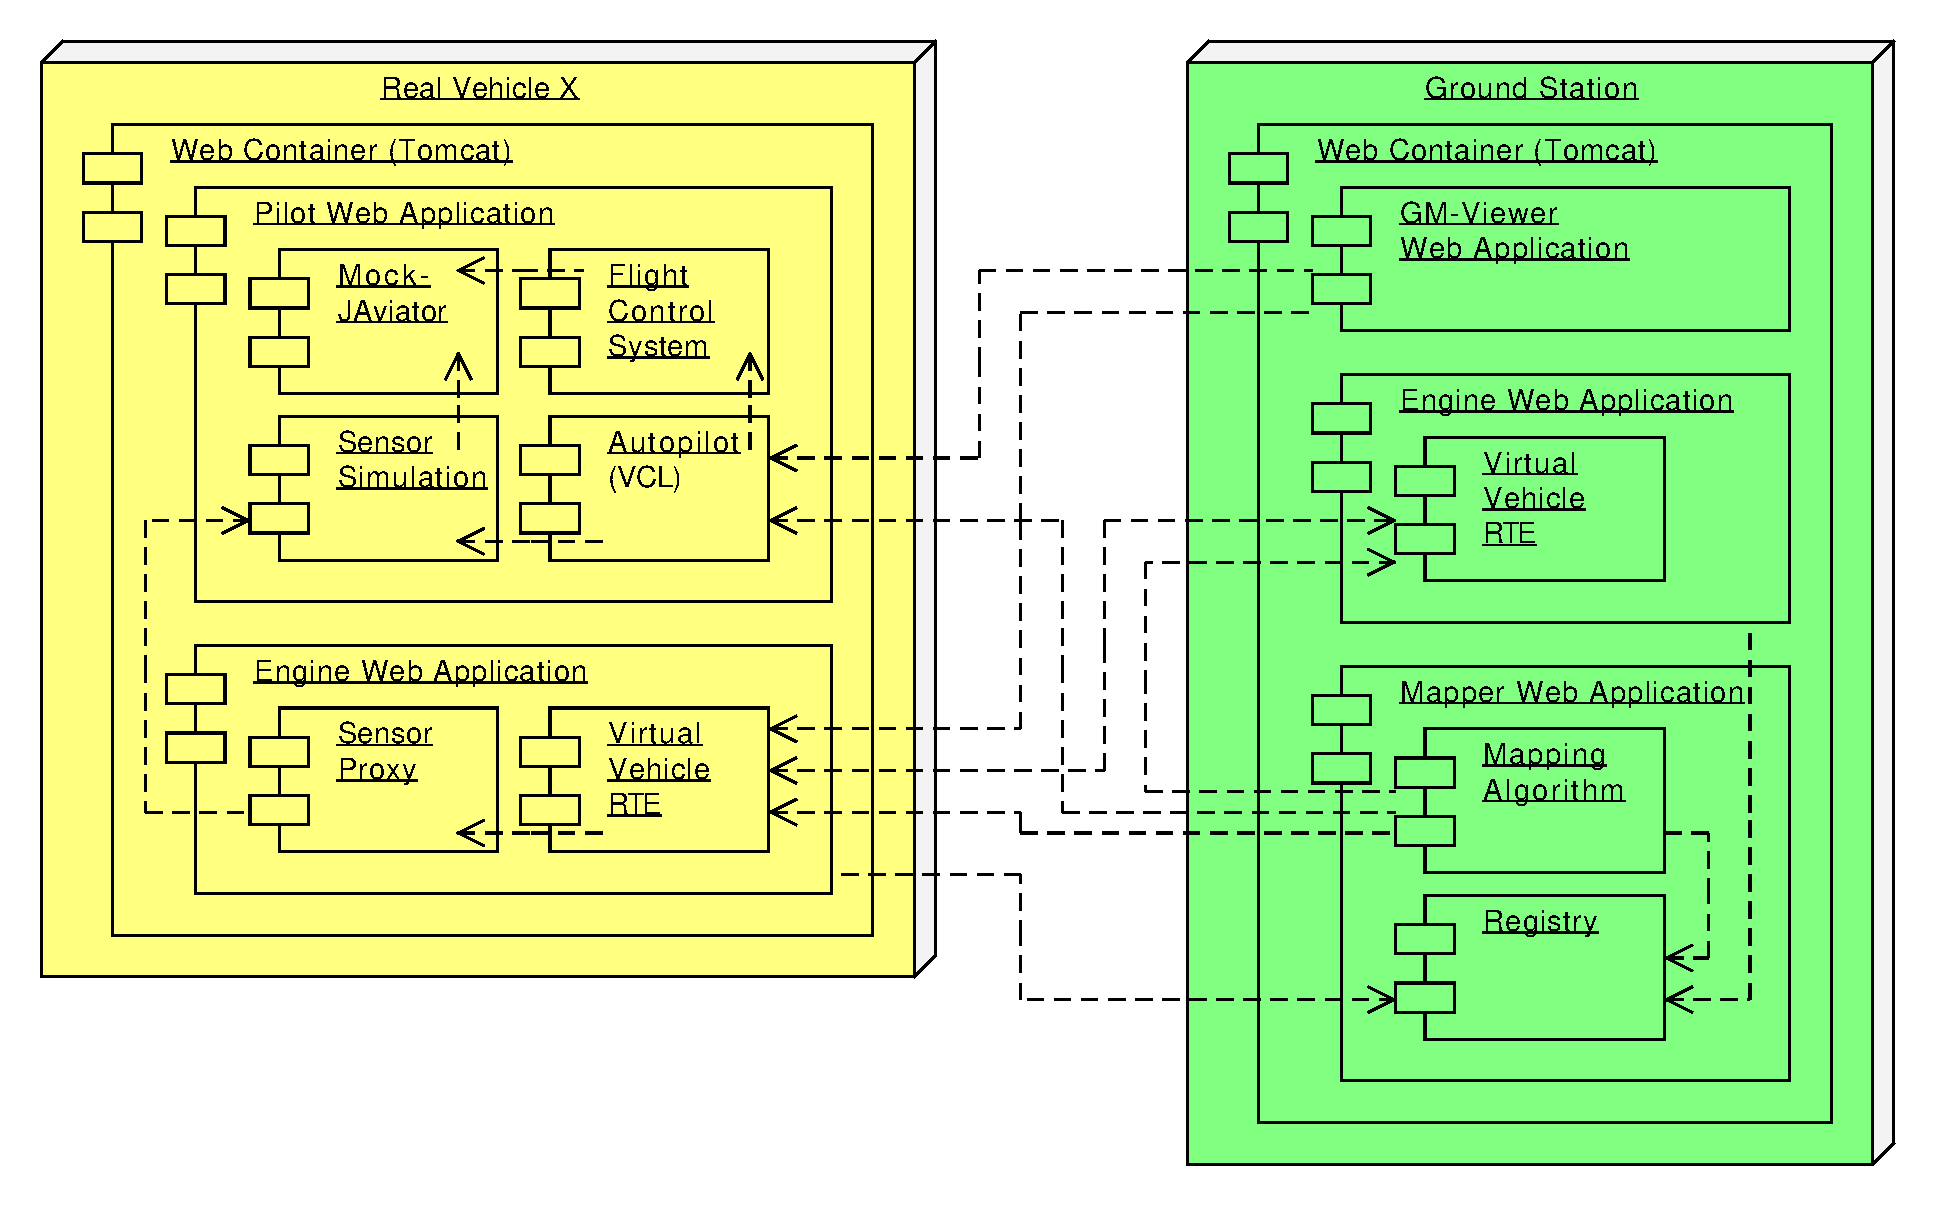
\includegraphics[width=10cm]{SystemOverview.pdf}}
        \end{center}
\end{frame}


\begin{frame}\frametitle{Simulator Overview}\framesubtitle{Sensors}
        \begin{center}
                {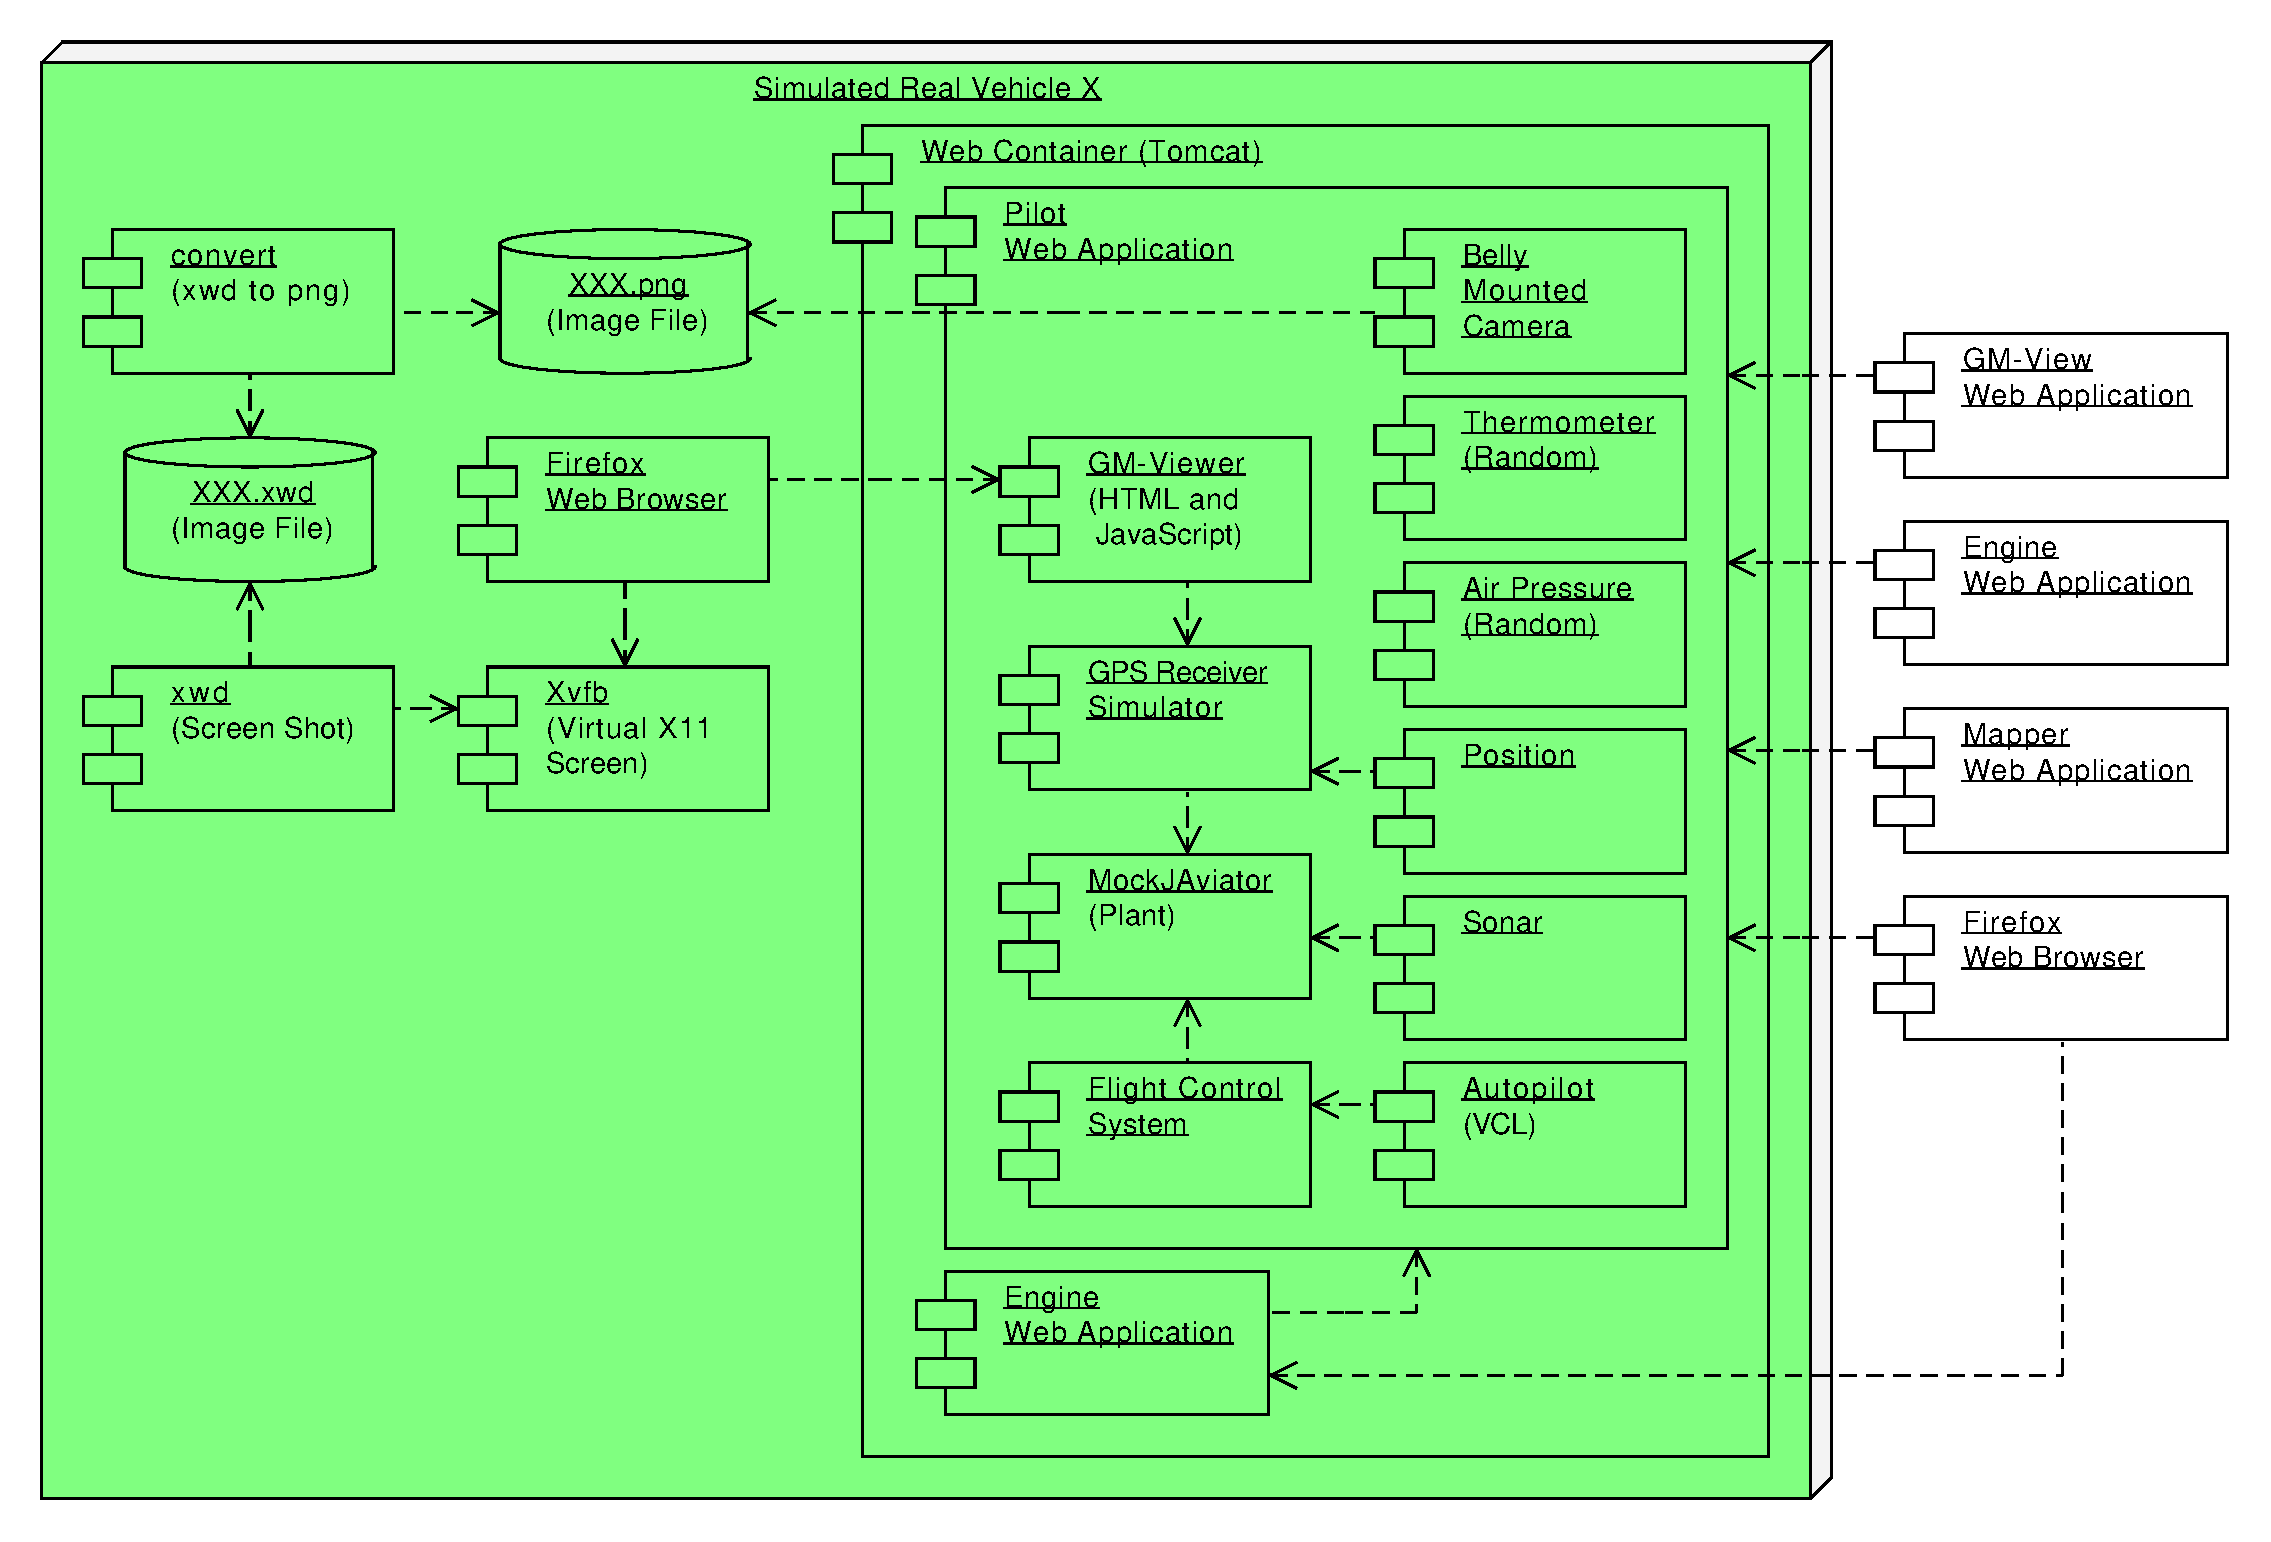
\includegraphics[width=10cm]{SensorSimulation-3.pdf}}
        \end{center}
\end{frame}




\section{Real Vehicles}
\begin{frame}\frametitle{Real Vehicles}\framesubtitle{Vehicle Configuration}
plant.simulated = true \\
plant.type = MockJAviator \\
plant.listener = udp://localhost:9011 \\
plant.location.system.type = gpssim \\
plant.location.system.listener = tcp://localhost:9012 \\
plant.location.system.update.rate = 10 \\
\quad \\
controller.simulated = true \\
controller.type = JControl \\
\quad \\
pilot.type = JPilot \\
pilot.name = Heli One \\
pilot.controller.connector = udp://localhost:9014
\end{frame}


\begin{frame}\frametitle{Real Vehicles}\framesubtitle{Sensor Configuration}
sensor.list = gps, temp, photo \\
\quad \\
sensor.gps.name = GPS receiver \\
sensor.gps.path = position \\
sensor.gps.uri = gps:/// \\
\quad \\
sensor.temp.name = thermometer \\
sensor.temp.path = temperature \\
sensor.temp.uri = rand:///18/22 \\
\quad \\
sensor.photo.name = belly mounted photo camera \\
sensor.photo.path = photo \\
sensor.photo.uri = x11:///:21
\end{frame}


\begin{frame}\frametitle{Real Vehicles}\framesubtitle{Vehicle Control Language}
\# \\
\# @(\#) real vehicle set course \\
\# \\
go auto \\
takeoff 1m for 5s \\
fly to (47.82204197, 13.04086670, 20.0)abs precision 1m 2.0mps \\
fly to (47.82206088, 13.04092035, 20.0)abs precision 1m 2.0mps \\
fly to (47.82195102, 13.04488063, 20.0)abs precision 1m 2.0mps \\
hover for 20s \\
land \\
go manual
\end{frame}





\section{Virtual Vehicles}
\begin{frame}\frametitle{Virtual Vehicles}

Virtual vehicles
\begin{itemize}
  \item run in the engine's virtual vehicle RTE as separate threads
  \item do the actual information aquisition
\end{itemize}

\vspace{0.5cm}
\pause

A virtual vehicle is a ZIP file containing
\begin{itemize}
  \item a task list,
  \item collected data as files,
  \item a virtual vehicle log file, and
  \item virtual vehicle specific properties
\end{itemize}

\end{frame}

\definecolor{zeit}{HTML}{BB8822}
\definecolor{wert}{HTML}{00AA22}
\begin{frame}\frametitle{Virtual Vehicles}\framesubtitle{Task List}
Point  ~47.82214552  ~13.04213136  ~20.0  ~tolerance  ~3.0 \\
Picture (\textcolor{zeit}{1327882656271} \textcolor{wert}{"img595205693794284171.png"}) \\
Temperature (\textcolor{zeit}{1327882768300} \textcolor{wert}{21.3}) \\
\quad \\
Point  ~47.82203567  ~13.04224133  ~20.0  ~tolerance  ~3.0 \\
Airpressure \\
\quad \\
Point  ~47.82196903  ~13.04228157  ~20.0  ~tolerance  ~3.0 \\
Picture
\end{frame}


\section{Mapping}
\begin{frame}\frametitle{Mapping} % \framesubtitle{}
Mapper
\begin{itemize}
  \item knows every engine and pilot web application
  \item maps virtual vehicles to physical vehicles
  \item initiates migration of virtual vehicles among
  	engines \\ (based on flight plans and available sensors) 
\end{itemize}

\begin{center}
        {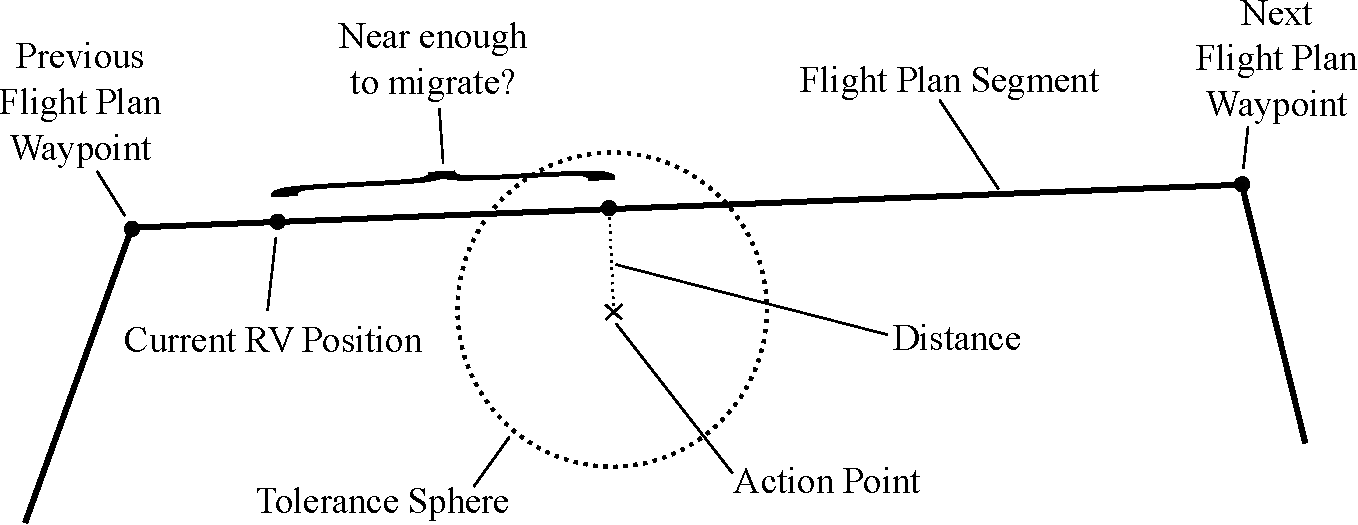
\includegraphics[width=10cm]{mapping.pdf}}
\end{center}
\end{frame}




\section{Demonstration}
\begin{frame}\frametitle{Demonstration} % \framesubtitle{}
	\begin{itemize}
	  \item two helicopters
	  \item one virtual vehicle
	  \item five photos
	\end{itemize}
	\vspace{0.5cm}

	\begin{center}
	        {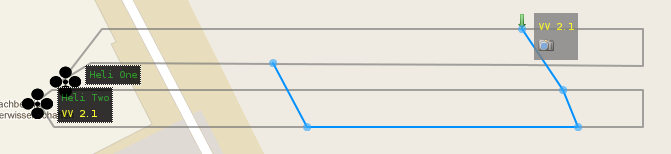
\includegraphics[width=10cm]{demo2-new.png}}
	\end{center}
\end{frame}


\end{document}
